%%%%%%%%%%%%%%%%%%%%%%%%%%%%%%%%%%%%%%%%%
% Beamer Presentation
% LaTeX Template
% Version 1.0 (10/11/12)
%
% This template has been downloaded from:
% http://www.LaTeXTemplates.com
%
% License:
% CC BY-NC-SA 3.0 (http://creativecommons.org/licenses/by-nc-sa/3.0/)
%
%%%%%%%%%%%%%%%%%%%%%%%%%%%%%%%%%%%%%%%%%

%----------------------------------------------------------------------------------------
%	PACKAGES AND THEMES
%----------------------------------------------------------------------------------------

\documentclass{beamer}
\usepackage[T1]{fontenc}
\usepackage{lmodern}
\usepackage[utf8]{inputenc}
\usepackage[german]{babel}
\usepackage[11pt]{moresize}

\usepackage{csquotes}       % provides \enquote{} macro for "quotes"

\mode<presentation> {

% The Beamer class comes with a number of default slide themes
% which change the colors and layouts of slides. Below this is a list
% of all the themes, uncomment each in turn to see what they look like.

%\usetheme{default}
%\usetheme{AnnArbor}
%\usetheme{Antibes}
%\usetheme{Bergen}
%\usetheme{Berkeley}
\usetheme{Berlin}
%\usetheme{Boadilla}
%\usetheme{CambridgeUS}
%\usetheme{Copenhagen}
%\usetheme{Darmstadt}
%\usetheme{Dresden}
%\usetheme{Frankfurt}
%\usetheme{Goettingen}
%\usetheme{Hannover}
%\usetheme{Ilmenau}
%\usetheme{JuanLesPins}
%\usetheme{Luebeck}
%\usetheme{Madrid}
%\usetheme{Malmoe}
%\usetheme{Marburg}
%\usetheme{Montpellier}
%\usetheme{PaloAlto}
%\usetheme{Pittsburgh}
%\usetheme{Rochester}
%\usetheme{Singapore}
%\usetheme{Szeged}
%\usetheme{Warsaw}

% As well as themes, the Beamer class has a number of color themes
% for any slide theme. Uncomment each of these in turn to see how it
% changes the colors of your current slide theme.

%\usecolortheme{albatross}
%\usecolortheme{beaver}
%\usecolortheme{beetle}
%\usecolortheme{crane}
%\usecolortheme{dolphin}
%\usecolortheme{dove}
%\usecolortheme{fly}
%\usecolortheme{lily}
%\usecolortheme{orchid}
%\usecolortheme{rose}
%\usecolortheme{seagull}
%\usecolortheme{seahorse}
%\usecolortheme{whale}
%\usecolortheme{wolverine}

%\setbeamertemplate{footline} % To remove the footer line in all slides uncomment this line
%\setbeamertemplate{footline}[page number] % To replace the footer line in all slides with a simple slide count uncomment this line

%\setbeamertemplate{navigation symbols}{} % To remove the navigation symbols from the bottom of all slides uncomment this line
}

\usepackage{graphicx} % Allows including images
\usepackage{booktabs} % Allows the use of \toprule, \midrule and \bottomrule in tables

%----------------------------------------------------------------------------------------
%	TITLE PAGE
%----------------------------------------------------------------------------------------

\title[Qualitätssicherungsphase]{Praxis der Softwareentwicklung\\ Qualitätssicherungsphase} % The short title appears at the bottom of every slide, the full title is only on the title page

%\author{Phasenverantwortlicher: } % Your name
\institute[PSE] % Your institution as it will appear on the bottom of every slide, may be shorthand to save space
{

}
\date{12. März 2018} % Date, can be changed to a custom date

\begin{document}

\begin{frame}
\titlepage % Print the title page as the first slide
\end{frame}

%\begin{frame}
%\frametitle{Overview} % Table of contents slide, comment this block out to remove it
%\tableofcontents % Throughout your presentation, if you choose to use \section{} and \subsection{} commands, these will automatically be printed on this slide as an overview of your presentation
%\end{frame}

%----------------------------------------------------------------------------------------
%	PRESENTATION SLIDES
%----------------------------------------------------------------------------------------

%------------------------------------------------
\section{Übersicht} 

\begin{frame}
\frametitle{Zeitlicher Ablauf}
\begin{itemize}
    \item Tests auf Paket- oder Klassenebene (Komponententest)
    \item Testen des Gesamtprodukts (paketübergreifend)
    \item Testen der Benutzeroberfläche
    \begin{itemize}
        \item Nutzerstudie
    \end{itemize}
\end{itemize}
\end{frame}

\begin{frame}
\frametitle{Architektur}
\begin{figure}
\centering
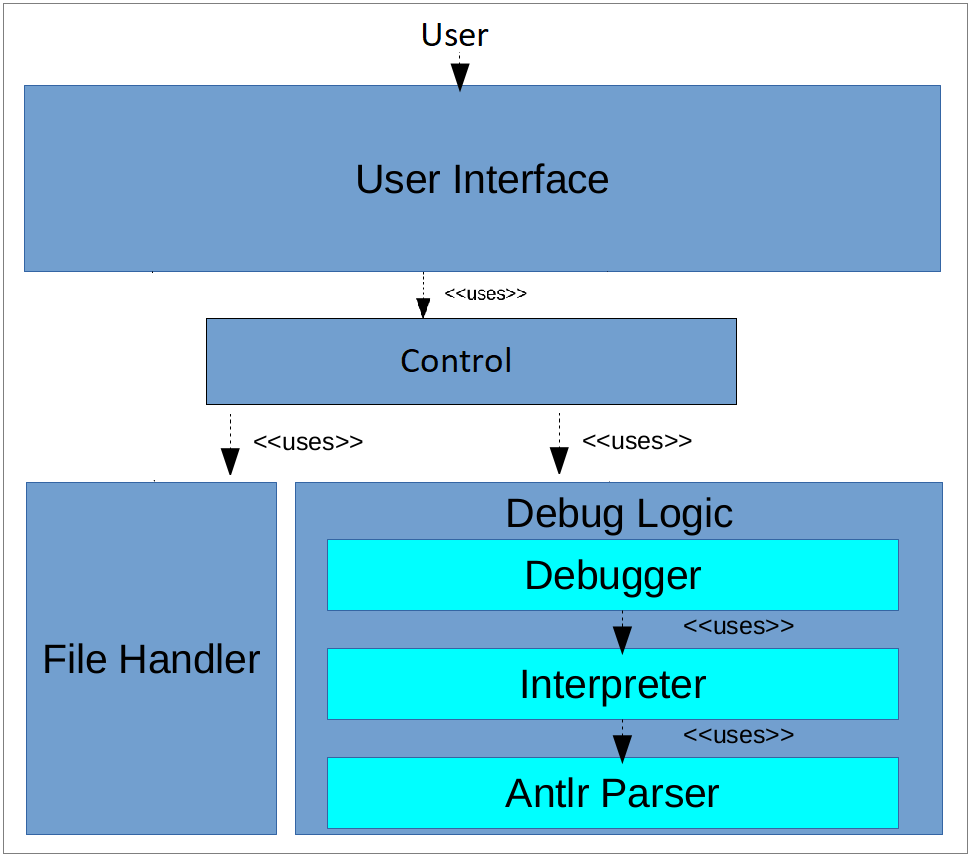
\includegraphics[width=0.5\textwidth]{../../Plichtenheft/Architektur.png}
\end{figure}
\end{frame}
%------------------------------------------------

%------------------------------------------------
\section{Testen einzelner Pakete} 

\begin{frame}
\frametitle{Durch JUnit-Tests erzielte Abdeckung}
\begin{figure}
\centering
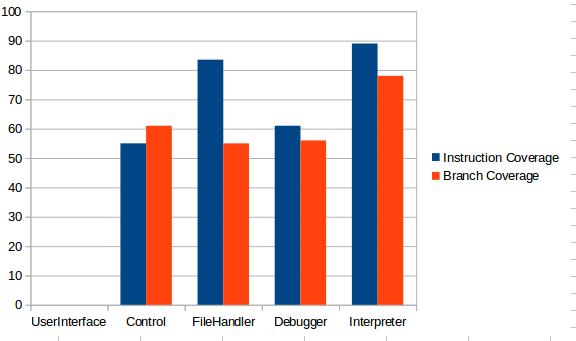
\includegraphics[width=0.8\textwidth]{../paketeCoverage.png}
\end{figure}
\end{frame}

\subsection{Interpreter}

\begin{frame}
\frametitle{Komponente = Klasse}
\begin{itemize}
    \item Testen der TermValues
    \item Testen der Terme
    \item Testen der Commands
    \item Testen der Visitor-Klassen
\end{itemize}
\end{frame}

\begin{frame}
\frametitle{Komponente = Paket}
\begin{itemize}
    \item Randfälle
    \begin{itemize}
        \item Syntax von Programmtexten, Watch-Expressions, Haltepunkten
        \item Semantik von Programmtexten, Watch-Expressions, Haltepunkten
    \end{itemize}
\end{itemize}
\end{frame}

\subsection{Control}
\begin{frame}
\frametitle{Laden von Konfigurationsdateien}
\begin{figure}
\centering
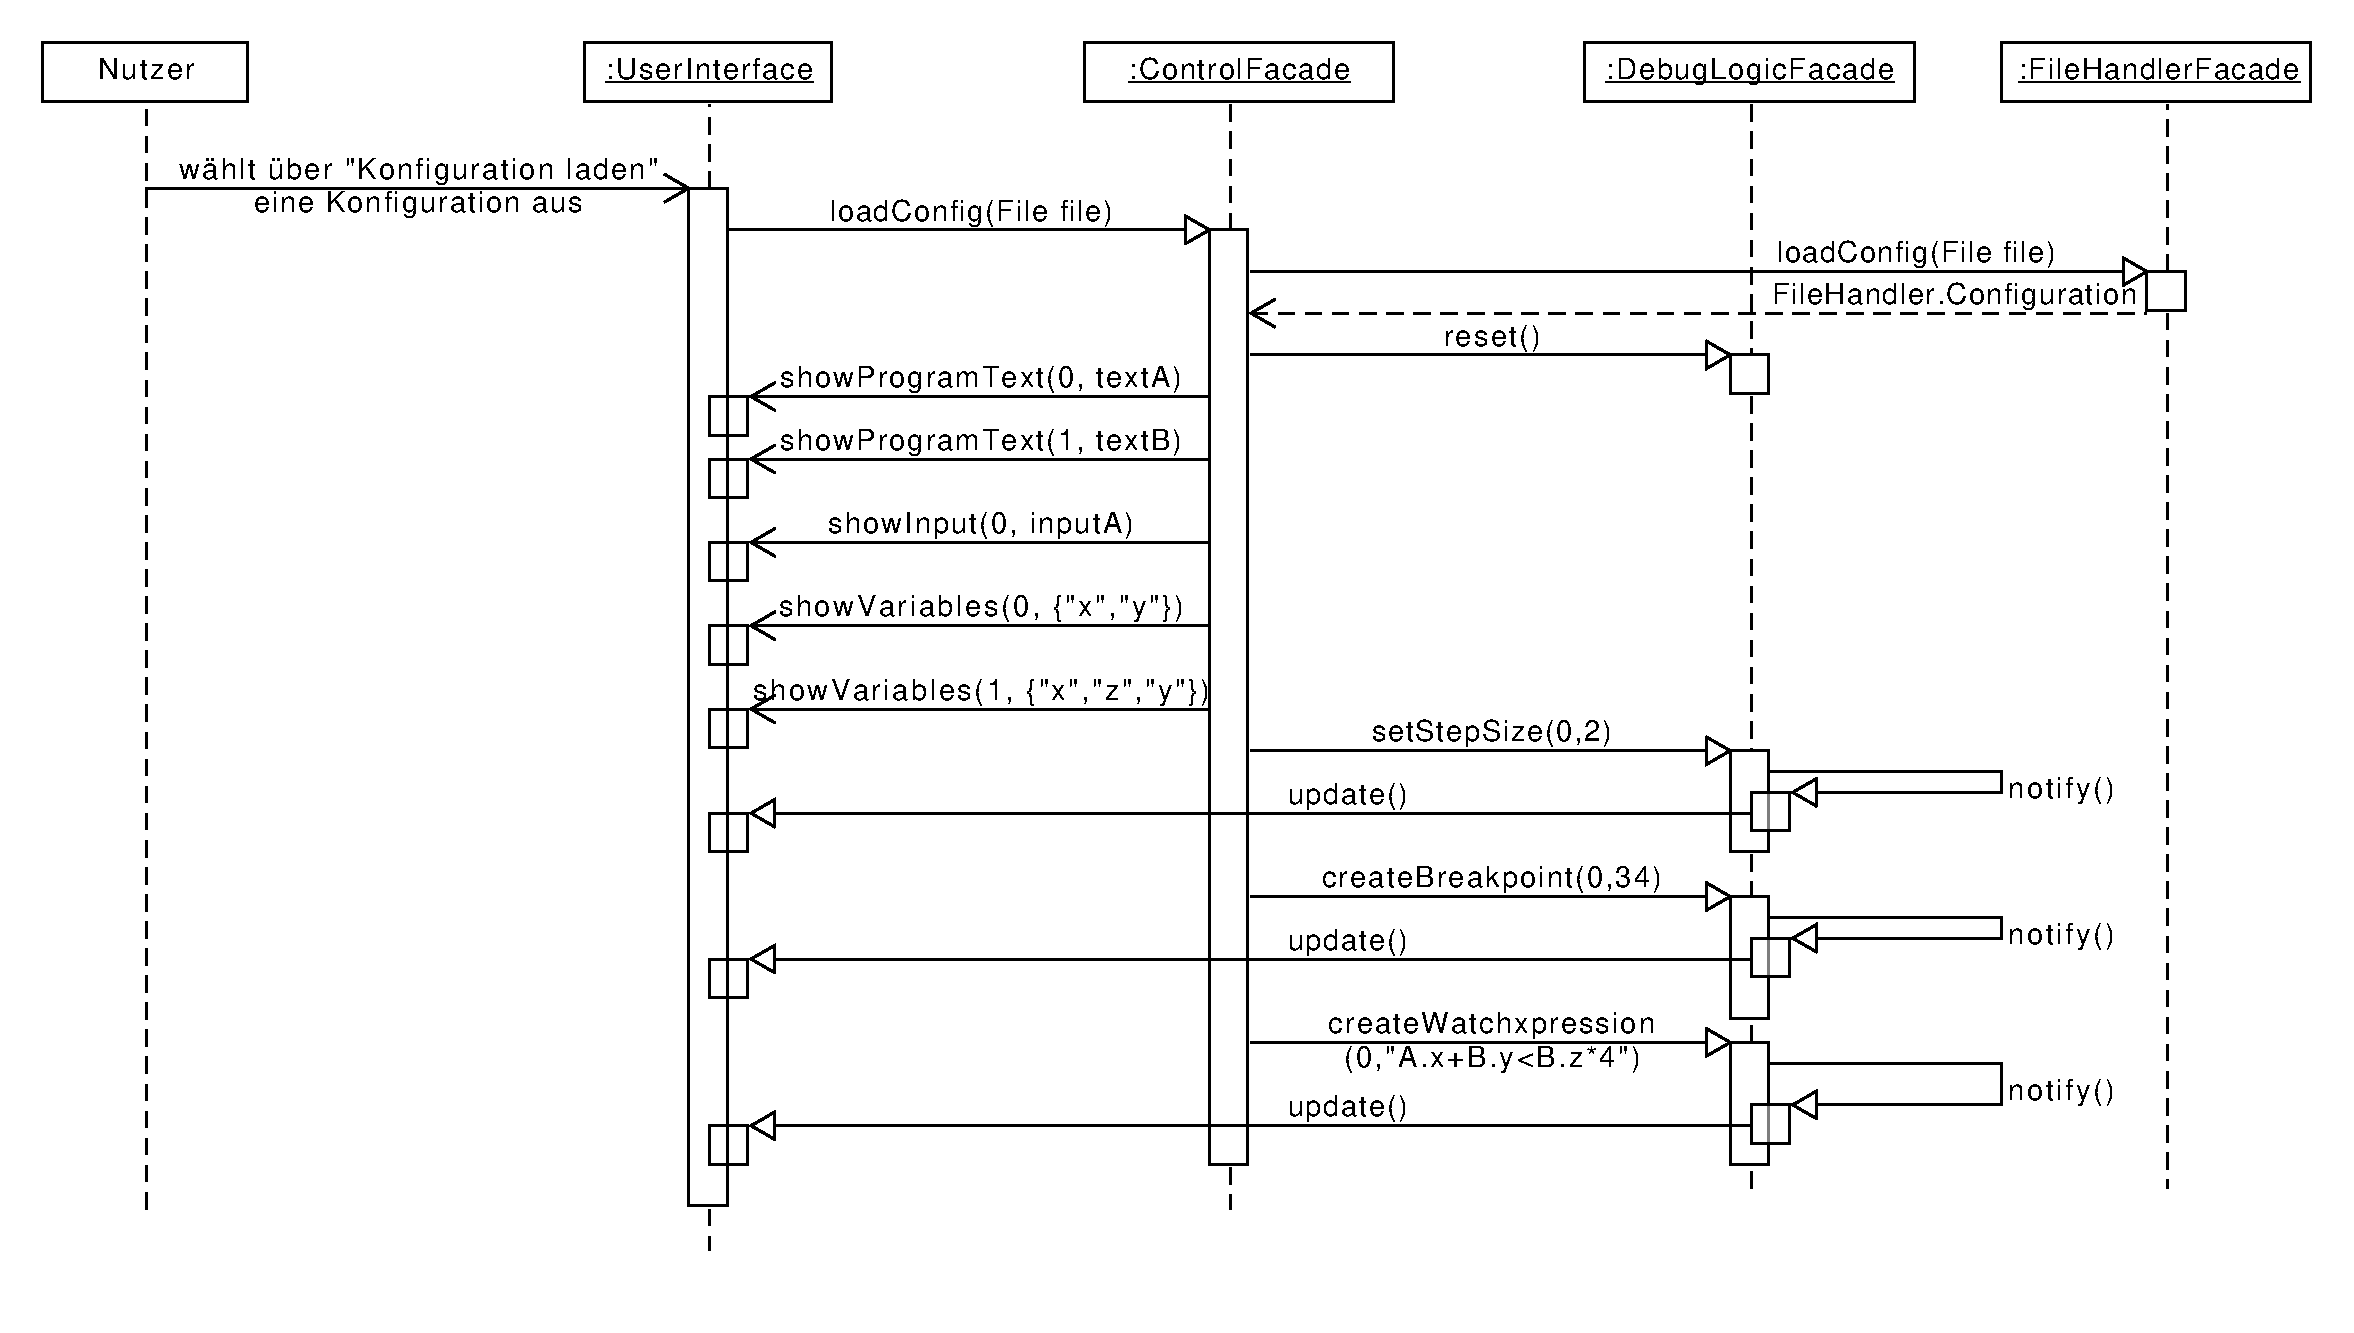
\includegraphics[width=1\textwidth]{../../Enwurf/diagrammIdeenUmlet/SequenceDiagrams/seq_loadConfigPDF.pdf}
\end{figure}
\end{frame}
%------------------------------------------------

%------------------------------------------------
\section{Testen der Benutzeroberfläche} 

\begin{frame}
\frametitle{Testverfahren}
\begin{itemize}
    \item Monkey Tests
    \item Testszenarien
    \begin{itemize}
        \item AF50
        \begin{itemize}
            \item Programm lässt sich über \textit{Programm hinzufügen} oder \textit{Programm öffnen} einbinden
            \item [...]
            \item Der Debugmodus lässt sich starten
            \item Schritte, Einzelschritte, etc. lassen sich ausführen 
            \item [...]
        \end{itemize}
    \end{itemize}
\end{itemize}
\end{frame}

\begin{frame}
\frametitle{Benutzerstudie}
\begin{itemize}
    \item Qualitätsanforderungen aus Pflichtenheft: Übersichtlichkeit, Verständlichkeit, Erlernbarkeit
    \item Acht Testpersonen
    \item Acht Aufgaben zum Testen der DIbugger-Konzepte (z.B. Nutzen der Menuleiste, Anordnung und Aufruf von Funktionen)
    \item Lautes Denken
\end{itemize}
\end{frame}
%------------------------------------------------

%------------------------------------------------
\section{Testen des Gesamtproduktes} 

\begin{frame}
\frametitle{Funktionale Tests}
\begin{itemize}
    \item Im Rahmen der Benutzeroberflächentests und weitere Szenarien zu ...
    \begin{itemize}
        \item Den Funktionalen Anforderungen aus dem Pflichtenheft
        \item Den Globalen Testfällen aus dem Pflichtenheft
    \end{itemize}
\end{itemize}
\end{frame}

\begin{frame}
\frametitle{Laufzeit und Speicherverbrauch}
\begin{itemize}
    \item Größte Rechenzeit:
    \begin{itemize}
        \item Aktualisieren der Benutzeroberfläche
        \item Methoden zur \enquote{Trace}-Erzeugung
    \end{itemize}
    \item Größter Speicherverbrauch:
    \begin{itemize}
        \item Programmbereiche der Benutzeroberfläche
        \item \textit{IntValue}, \textit{TraceState}
    \end{itemize}
\end{itemize}
\end{frame}
%------------------------------------------------

\end{document} 
